\documentclass{article}
% Change "article" to "report" to get rid of page number on title page
\usepackage{amsmath,amsfonts,amsthm,amssymb}
\usepackage{algorithmic,algorithm}
\usepackage{setspace}
\usepackage{Tabbing}
\usepackage{fancyhdr}
\usepackage{lastpage}
\usepackage{extramarks}
\usepackage{chngpage}
\usepackage{soul,color}
\usepackage{ulem}
\usepackage{graphicx,float,wrapfig}
\usepackage{pifont}
\usepackage{booktabs}
\usepackage{hyperref}
\usepackage{pstricks,pst-node,pst-tree}
\usepackage{pdftricks}
\usepackage{subfigure}
\usepackage{multicol}
\usepackage{enumerate}
\usepackage{multirow}

\usepackage{listings}
\usepackage{color}
\usepackage{textcomp}
\definecolor{listinggray}{gray}{0.9}
\definecolor{lbcolor}{rgb}{0.9,0.9,0.9}
\lstset{
  % backgroundcolor=\color{lbcolor},
  tabsize=4,
  rulecolor=,
  language=c++,
  basicstyle=\setstretch{1},
  upquote=true,
  aboveskip={\baselineskip},
  columns=fixed,
  showstringspaces=false,
  extendedchars=true,
  breaklines=true,
  prebreak = \raisebox{0ex}[0ex][0ex]{\ensuremath{\hookleftarrow}},
  % frame=single,
  showtabs=false,
  showspaces=false,
  showstringspaces=false,
  identifierstyle=\ttfamily,
  keywordstyle=\color[rgb]{0,0,1},
  commentstyle=\color[rgb]{0.133,0.545,0.133},
  stringstyle=\color[rgb]{0.627,0.126,0.941},
}
% In case you need to adjust margins:
\topmargin=-0.45in      %
\evensidemargin=0in     %
\oddsidemargin=0in      %
\textwidth=7.0in        %
\textheight=9.2in       %
\headsep=0.25in         %

% Homework Specific Information
\newcommand{\hmwkTitle}{Homework\ \#3}
\newcommand{\hmwkDueDate}{Oct.\ 12th,\ 2010}
\newcommand{\hmwkClass}{Data Structure}
\newcommand{\hmwkClassTime}{TR\ 4:10-5:25pm}
\newcommand{\hmwkClassInstructor}{Meilin\ Liu}
\newcommand{\hmwkAuthorName}{Shumin\ Guo}
\newcommand{\answer}{\textbf{\\\underline{ANSWER:}\\}}

% Setup the header and footer
\pagestyle{fancy}                                                       %
\lhead{\hmwkAuthorName}                                                 %
\chead{\hmwkClass\ - \hmwkTitle}  %
\rhead{Page\ \thepage\ of\ \pageref{LastPage}}                          %
\lfoot{\lastxmark}                                                      %
\cfoot{}                                                                %
\rfoot{}                          %
\renewcommand\headrulewidth{0.4pt}                                      %
%\renewcommand\footrulewidth{0.2pt}                                     %

%%%%%%%%%%%%%%%%%%%%%%%%%%%%%%%%%%%%%%%%%%%%%%%%%%%%%%%%%%%%%
% Make title
\title{\textmd{\textbf{\hmwkClass:\
      \hmwkTitle}}\\\normalsize\small{Due\ Date:\
    \hmwkDueDate}\\} 
\date{\today}
\author{\textsc{\hmwkAuthorName}}
%%%%%%%%%%%%%%%%%%%%%%%%%%%%%%%%%%%%%%%%%%%%%%%%%%%%%%%%%%%%%

\begin{document}
\begin{center}
\textbf{{\LARGE CS 400/600  Homework \#3} \\
Due Date: Oct. 28th, 2010, beginning of the class.}
\end{center}

\begin{enumerate}
\item(10 points) Draw the 11-item hash table that results from using
  the hash function $h(k)= k \% 11$. To hash the keys 10, 22, 31, 4,
  15, 28, 17, 88, and 59, assuming collisions are handled by
  chaining. 
\answer Please see the hash key and value table at Table
\ref{tbl:hashvalue}
\begin{table}[H]
  \begin{center}
    \begin{tabular}{|c|c|c|c|c|c|c|c|c|c|} 
      \hline Hash Key(k)&10&22&31&4&15&28&17&88&59 \\
      \hline $h(k)=k\%11$&10&0 &9 &4&4 &6 &6 &0 &4 \\
      \hline
    \end{tabular}
    \caption{Hash Key and Hash Value Reference
      Table($h(k)=k\%11$). \label{tbl:hashvalue}}  
    \vspace{-15pt}
  \end{center}
\end{table}
With open chaining hashing, the result is shown in Figure
\ref{tbl:chainhash} \\ 

\begin{figure}[H]
  \vspace{-15pt}
  \begin{center}
    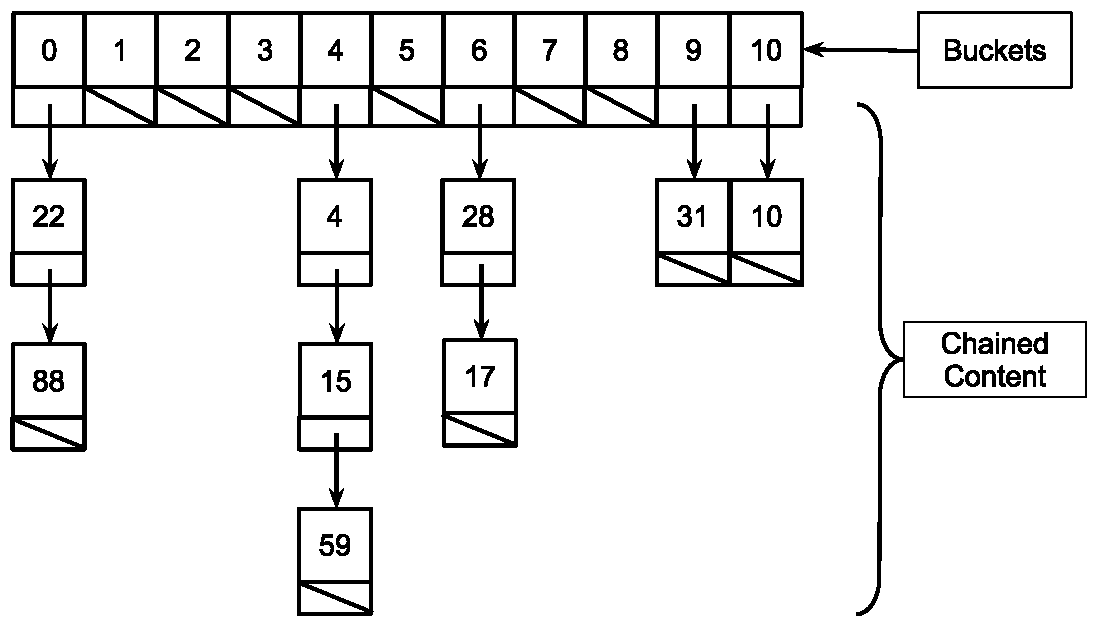
\includegraphics[scale=0.7]{chained_hashing}
    \caption{Hash Key layout with open Chain
      Hashing. \label{tbl:chainhash}}
    \vspace{-15pt}
  \end{center}
\end{figure}

\item(20 points) What is the result of question 1, assuming collisions
  are handled by linear probing.
\answer With linear probing, we will have probing steps $0, 1, 2, 3,
\ldots i$. \\
Please reference the hash value table at Table
\ref{tbl:hashvalue} and the Linear hash result at Table
\ref{tbl:linearhash} 

\begin{table}[H]
  \begin{center}
    \begin{tabular}{|c|c|c|c|c|c|c|c|c|c|c|c|} 
      \hline Bucket(Slot)&0&1&2&3&4&5&6&7&8&9&10 \\
      \hline 
      Content &22&88& & &4&15&28&17&59&31&10 \\
      \hline
    \end{tabular}
    \caption{Hash Key layout with closed hash, linear
      probing. \label{tbl:linearhash}}
    \vspace{-15pt}
  \end{center}
\end{table}
$\sum_1^{m+1}100i$
\item(10 points). Show the result of question 1, assuming collisions
  are handled by quadratic probing (the probe function $p(k,i) = i^2$,
  i is called probe number, $i=0, 1,\ldots N-1$ ),  up to the point where
  the method fails because no empty slot is found. 
\answer With quadratic probing, we will have probing steps $0, 1, 4, 9,
\ldots i^2$. \\
Please reference the hash value table at Table
\ref{tbl:hashvalue} and the Linear hash result at Table \ref{tbl:quadhash}
\begin{table}[H]
  \begin{center}
    \begin{tabular}{|c|c|c|c|c|c|c|c|c|c|c|c|} 
      \hline Bucket(Slot)&0&1&2&3&4&5&6&7&8&9&10 \\
      \hline 
      Content &22&88& & &4&15&28&17&59&31&10 \\
      \hline
    \end{tabular}
    \caption{Hash Key layout with closed hash, quadratic
      probing. \label{tbl:quadhash}}
    \vspace{-15pt}
  \end{center}
\end{table}

\item(10 points). What is the result of question 1 assuming collisions
  are handled by double hashing using a secondary hash function 
  $h^\prime (k) = 1 + (k \% (m-1))$?
\answer With double hashing, we have the hash function:
$h(k,j)=(h_1(k)+j.h_2(k))\%m$, of which $h_1(k)$ is the main hash
function and $h_2(k)$ is the secondary hash function, and k is the
hash key and j is the probing steps respectively. \\
Please reference the hash value table at Table
\ref{tbl:hashvalue}, the hash value table of the secondary hash
function at Table \ref{tbl:sechashvalue} and the double hashing result at
Table \ref{tbl:doublehash} 

\begin{table}[H]
  \begin{center}
    \begin{tabular}{|c|c|c|c|c|c|c|c|c|c|c|c|} 
      \hline Secondary Hash Key(k) &10&22&31&4&15&28&17&88&59 \\
      \hline $h^\prime(k)=1+(k\%(m-1))$&1&3&2&5&6&9&8&9&10 \\
      \hline
    \end{tabular}
    \caption{Secondary Hash Key and Value Reference Table. \label{tbl:sechashvalue}} 
    \vspace{-15pt}
  \end{center}
\end{table}

\begin{table}[H]
  \begin{center}
    \begin{tabular}{|c|c|c|c|c|c|c|c|c|c|c|c|} 
      \hline Bucket(Slot)&0&1&2&3&4&5&6&7&8&9&10 \\
      \hline 
      Content &22& &59&17&4&15&28&88& &31&10 \\
      \hline
    \end{tabular}
    \caption{Hash Key layout with closed double
      hashing. \label{tbl:doublehash}} 
    \vspace{-15pt}
  \end{center}
\end{table}


\item(30 points). Consider the following AVL tree:\\
\begin{figure}[H]
  \vspace{-10pt}
  \begin{center}
    \pstree[levelsep=5ex]{\Tcircle{10} }{
      \pstree{ \Tcircle{5}}{ % level - 1
        \Tcircle{1}\Tn
      }
      \pstree{\Tcircle{20}} {
        \Tcircle{15}
        \pstree{\Tcircle{30}} {
          \Tcircle{25}
          \Tcircle{40}
        }
      }
    }
    \caption{AVL Tree.\label{fig:question5}}
    \vspace{-15pt}
  \end{center}
\end{figure}


\begin{enumerate}[(1)]
\item Suppose that the value 21 were inserted into the above tree.
  Draw the rebalanced AVL tree. 
\answer After rebalance we will get the balanced tree as in Figure
\ref{fig:insertrebalanced}
\begin{figure}[H]
  \vspace{-10pt}
  \begin{center}
    \pstree[levelsep=5ex]{\Tcircle{10} }{
      \pstree{\Tcircle{5}}{ % level - 1
        \Tcircle{1}\Tn
      }
      \pstree[levelsep=5ex]{\Tcircle{25} }{
        \pstree{\Tcircle{20}}{ % level - 1
          \Tcircle{15}
          \Tcircle{21}
        }
        \pstree{\Tcircle{30}} {
          \Tn\Tcircle{40}
        }
      }
    }
    
    \caption{Rebalanced Tree After Inserting 21.\label{fig:insertrebalanced}}
    \vspace{-15pt}
  \end{center}
\end{figure}


\item with the result from (1), the node labeled with "1" is
  removed. Please draw the re-balanced tree after deletion.
\answer After rebalance we will get the balanced tree as in Figure
\ref{fig:deleterebalanced}
\begin{figure}[H]
  \vspace{-10pt}
  \begin{center}
    \pstree[levelsep=5ex]{\Tcircle{25} }{
      \pstree{\Tcircle{10}}{ % level - 1
        \Tcircle{5}\Tn
        \pstree{\Tcircle{20}} {
          \Tcircle{15}
          \Tcircle{21}
        }
      }
      \Tn\pstree{\Tcircle{30}} {
        \Tn\Tcircle{40}
      }
    }
    \caption{Rebalanced Tree After Deleting 1.\label{fig:deleterebalanced}}
    \vspace{-15pt}
  \end{center}
\end{figure}



\end{enumerate}                 %question 5.

\end{enumerate}                 %the whole doc
\end{document}

%%%%%%%%%%%%%%%%%%%%%%%%%%%%%%%%%%%%%%%%%%%%%%%%%%%%%%%%%%%%%
